\section{Checking an adapted-reference watermark teacher}
\label{sec:transport_teacher}
The failed parameter-filter pilot motivates a function-space alternative: train the marked student after adaptation toward a marked version of an adapted clean reference. Section~\ref{app:transport} defines the adapted-reference target and its fixed-reference control. Before robustness training, a prerequisite is to check whether this teacher itself produces detectable, content-preserving marks.

We use the released clean UViT-H generator, DC-AE decoder and DistSeal latent embedder. The public model card supplies watermark strength $0.5$, applied in raw autoencoder latent units before decoding. Diffusion-generator latents are divided by $0.2889$ before embedding. The fixed teacher marks clean-model samples. The adapted teacher marks samples after 100 clean AdamW updates at learning rate $10^{-5}$, batch size four, using a frozen sequence drawn from the first 2,000 of the existing 8,000 fitting images. The owner detector does not enter this clean update. Indices 4,000--7,999 are reserved for later development removal training; teacher support does not overlap them. These partitions are new to this development comparison, not a claim of an untouched external benchmark.

Thirty-two fresh coupled generation seeds and labels from the existing 200-class fitting holdout are frozen before generation. The paired-quality reference is each teacher's own clean output, before applying the embedder. The initial screen requires at least 28/32 detections and 28/32 preservation passes per teacher, under the LPIPS, SSIM and CLIP limits in Section~\ref{sec:preservation}. The original owner threshold $>0.6875$ remains fixed.

\begin{table}[ht]\centering\small
\begin{tabular}{lrrrr}\toprule
Reference & Clean detected & Marked detected & Preserved & Mean LPIPS\\\midrule
Fixed & 0/32 & 32/32 & 31/32 & 0.0411\\
Adapted & 0/32 & 32/32 & 31/32 & 0.0396\\\bottomrule
\end{tabular}
\caption{Prerequisite teacher validation. Preservation compares the post-hoc marked image with its corresponding clean reference. These counts do not measure robustness of a distilled generator after a removal attack.}
\end{table}

Both teachers pass the screen. All 128 native PNG hashes, sample indices, class labels and preservation sums are verified against the saved records. The allocation uses 622 seconds on one H100, including a slow dependency startup and quality evaluation. A matched first-order meta-distillation comparison is launched separately; a trained model's initial quality, independent removal attacks, calibration and repeated-seed confirmation still require evaluation. No robustness gain is inferred from the table above.

\begin{figure}[p]\centering
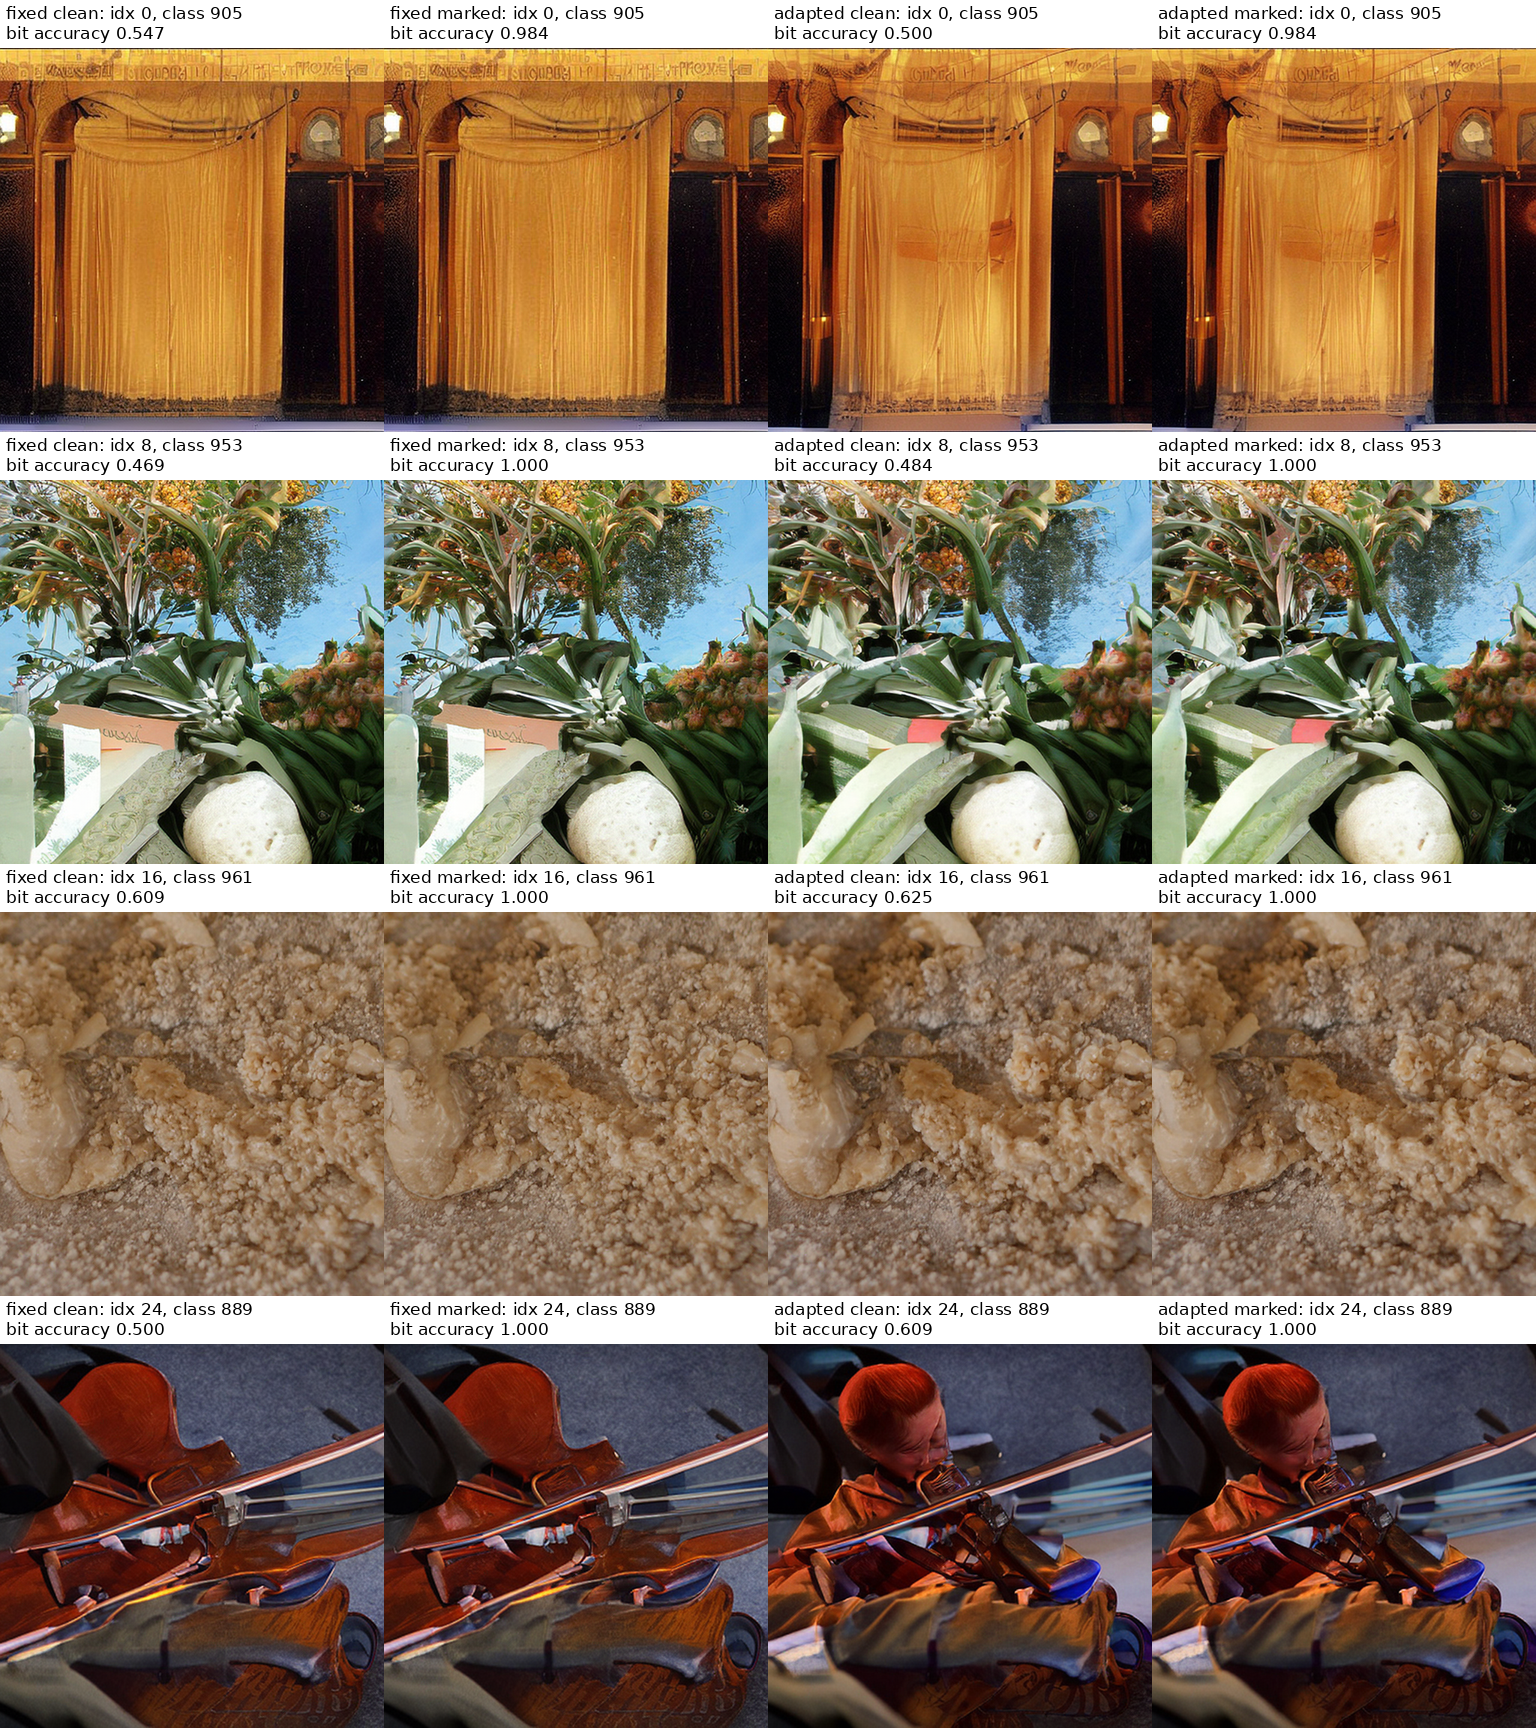
\includegraphics[width=\linewidth]{figures/transport-teacher.png}
\caption{The fixed and adapted references before and after post-hoc marking. Rows show positions 0, 8, 16 and 24, chosen after the run without filtering by detection or quality. The display is resized uniformly; native outputs are retained. Similarity of marking pairs is a different question from similarity between the two independently adapted generators.}
\end{figure}
